\subsection{Aufgabe 3}
\subsubsection{Aufbau}
Die Apparatur wurde aus Aufgabe 1 übernommen. Die Spaltbreite wurde auf \(0,2\,mm\) eingestellt und anschließend wurde der Messung begonnen.
\subsubsection{Durchführung}
Vermessen wurde als erstes die Indigo-Linie des Farbspektrums, da diese schon aus der vorherigen Aufgabe eingestellt war, anschließend folgten die grüne- und gelbe Linie. Die Gegenspannung \(U_G\) wurde langsam abgebaut und die gemessenen Ströme \(I_{Pho}\) notiert. Die Messabstände wurden so gewählt, dass bei relativ konstantem Verlauf nur wenig Messwerte genommen wurden, bei größeren Änderungen aber viele.
\subsubsection{Beobachtung}
Bis zu einer Gewissen Spannung trat kaum eine Änderung des Stroms \(I_{Pho}\) auf, anschließend jedoch sehr schnell. Bis zu einer gewssen Spannu ng stieg der Strom immer weiter blieb dann jedoch realtiv konstant. \newpage
\subsubsection{Messwerte}
\begin{center}
\begin{longtable}{c|c}
\(U_B [V]\) & \(I_{Pho} [pA]\)\\\hline \endhead
\(-8\) & \( -0.5\) \\ 
\(-7\) & \( -0.6\) \\ 
\(-6\) & \( -0.6\) \\ 
\(-5\) & \( -0.6\) \\ 
\(-4\) & \( -0.6\) \\ 
\(-3\) & \( -0.6\) \\ 
\(-2\) & \( -0.6\) \\ 
\(-1.5\) & \( -0.6\) \\ 
\(-1.1\) & \( -0.5\) \\ 
\(-1\) & \( -0.5\) \\ 
\(-0.9\) & \( -0.26\) \\ 
\(-0.8\) & \( -0.06\) \\ 
\(-0.7\) & \( 0.47\) \\ 
\(-0.6\) & \( 1.08\) \\ 
\(-0.5\) & \( 1.8\) \\ 
\(-0.4\) & \( 2.7\) \\ 
\(-0.3\) & \( 3.9\) \\ 
\(-0.2\) & \( 5.3\) \\ 
\(-0.1\) & \( 7\) \\ 
\(0\) & \( 8.95\) \\ 
\(0.2\) & \( 14.2\) \\ 
\(0.4\) & \( 19.8\) \\ 
\(0.6\) & \( 26\) \\ 
\(0.8\) & \( 32.6\) \\ 
\(1\) & \( 33.6\) \\ 
\(1.2\) & \( 42.9\) \\ 
\(1.4\) & \( 52.2\) \\ 
\(1.6\) & \( 60.3\) \\ 
\(1.8\) & \( 69\) \\ 
\(2\) & \( 76.4\) \\ 
\(2.2\) & \( 84.2\) \\ 
\(2.4\) & \( 91.4\) \\ 
\(2.6\) & \( 98.4\) \\ 
\(2.8\) & \( 104\) \\ 
\(3\) & \( 112\) \\ 
\(3.2\) & \( 118\) \\ 
\(3.4\) & \( 123\) \\ 
\(3.6\) & \( 127\) \\ 
\(3.8\) & \( 130\) \\ 
\(4\) & \( 135\) \\ 
\(4.5\) & \( 142\) \\ 
\(5\) & \( 148\) \\ 
\(5.5\) & \( 153\) \\ 
\(6\) & \( 157\) \\ 
\(6.5\) & \( 162\) \\ 
\(7\) & \( 167\) \\ 
\(7.5\) & \( 170\) \\ 
\(8\) & \( 174\) \\
\end{longtable}
\captionof{table}{Messwerte der Indigo-Linie}
\begin{longtable}{c|c}
\(U_B [V]\) & \(I_{Pho} [pA]\)\\\hline \endhead
\(-8\) & \( 0.2\) \\ 
\(-7.8\) & \( 0.1\) \\ 
\(-7.6\) & \( 0.1\) \\ 
\(-7.4\) & \( 0.05\) \\ 
\(-7.2\) & \( 0.06\) \\ 
\(-7\) & \( 0.04\) \\ 
\(-6.8\) & \( 0.06\) \\ 
\(-6.6\) & \( 0.05\) \\ 
\(-6\) & \( 0.05\) \\ 
\(-5\) & \( 0.03\) \\ 
\(-4\) & \( 0.04\) \\ 
\(-3\) & \( 0.1\) \\ 
\(-2\) & \( 0.16\) \\ 
\(-1\) & \( 0.2\) \\ 
\(-0.5\) & \( 0.25\) \\ 
\(0\) & \( 0.8\) \\ 
\(0.2\) & \( 1.7\) \\ 
\(0.4\) & \( 4.5\) \\ 
\(0.6\) & \( 10.3\) \\ 
\(0.8\) & \( 20.98\) \\ 
\(1\) & \( 39.4\) \\ 
\(1.2\) & \( 66.9\) \\ 
\(1.4\) & \( 106\) \\ 
\(1.6\) & \( 141\) \\ 
\(1.8\) & \( 175\) \\ 
\(2\) & \( 208\) \\ 
\(2.2\) & \( 242\) \\ 
\(2.4\) & \( 267\) \\ 
\(2.6\) & \( 286\) \\ 
\(2.8\) & \( 202\) \\ 
\(3\) & \( 316\) \\ 
\(3.2\) & \( 330\) \\ 
\(3.4\) & \( 341\) \\ 
\(3.6\) & \( 351\) \\ 
\(6.8\) & \( 359\) \\ 
\(4\) & \( 372\) \\ 
\(5\) & \( 391\) \\ 
\(6\) & \( 409\) \\ 
\(7.8\) & \( 419\) \\ 
\(8\) & \( 435\) \\
\end{longtable}
\captionof{table}{Messwerte der grünen Linie}
\begin{longtable}{c|c}
\(U_B [V]\) & \(I_{Pho} [pA]\)\\\hline \endhead
\(-8\) & \( 0.6\) \\ 
\(-7\) & \( 0.44 \) \\ 
\(-6\) & \( 0.35 \) \\ 
\(-5\) & \( 0.35 \) \\ 
\(-4\) & \( 0.32 \) \\ 
\(-3\) & \( 0.29 \) \\ 
\(-2\) & \( 0.33 \) \\ 
\(-1\) & \( 0.37 \) \\ 
\(0\) & \( 0.37 \) \\ 
\(0.6\) & \( 0.5 \) \\ 
\(0.8\) & \( 1.12 \) \\ 
\(1\) & \( 0.4 \) \\ 
\(1.2\) & \( 0.6\) \\ 
\(1.4\) & \( 1.9 \) \\ 
\(1.6\) & \( 7.44\) \\ 
\(1.8\) & \( 19.4 \) \\ 
\(2\) & \( 36.9 \) \\ 
\(2.2\) & \( 59.7 \) \\ 
\(2.4\) & \( 82.3 \) \\ 
\(2.6\) & \( 106.8 \) \\ 
\(2.8\) & \( 128 \) \\ 
\(3\) & \( 142 \) \\ 
\(3.2\) & \( 150\) \\ 
\(3.4\) & \( 157 \) \\ 
\(3.6\) & \( 162 \) \\ 
\(3.8\) & \( 165 \) \\ 
\(4\) & \( 169 \) \\ 
\(4.2\) & \( 172 \) \\ 
\(4.4\) & \( 174 \) \\ 
\(4.6\) & \( 176 \) \\ 
\(4.8\) & \( 177 \) \\ 
\(5\) & \( 178 \) \\ 
\(5.2\) & \( 179 \) \\ 
\(5.4\) & \( 180 \) \\ 
\(5.6\) & \( 182 \) \\ 
\(5.8\) & \( 182 \) \\ 
\(6\) & \( 183 \) \\ 
\(6.5\) & \( 190\) \\ 
\(7\) & \( 191 \) \\ 
\(7.5\) & \( 193\) \\ 
\(8\) & \( 196 \) \\
\end{longtable}
\captionof{table}{Messwerte bei der gelben Linie}
\end{center}
\subsubsection{Fehlerbetrachtung}
Die Fehler der Messung sind mit den vorhandenen Daten nur grob schätzbar, da es sich um selbstgebaute Geräte handelt gibt es keine Herstellerangaben. Außerdem ist der größte Anteil an Fehlern nicht statistischer sondern systematischer Natur und daher nicht mittels gaußscher Fehlerforpflanzung berechenbar. Es werden im folgenden folgende Fehler angenommen:
\begin{center}
\begin{tabular}{c|c}
Messgröße & Fehler \\\hline
\(d\) & \( 0,05\,mm\)\\
\(U_G\) & \( 0,01\,V\)\\
\(I_{Pho}\) & \( 1\, pA\)\\
\end{tabular}
\captionof{table}{Eingangsfehler}
\end{center}
\subsubsection{Graphen}
Die Daten werden nun graphisch aufgetragen, wobei die Kennlinien sichtbar werden:
\begin{center}
\begin{minipage}{\linewidth}
\centering
\makebox[0cm]{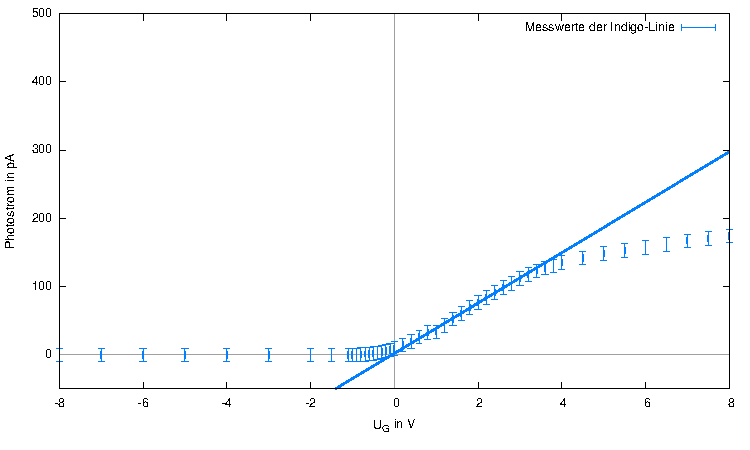
\includegraphics[width=\textwidth]{graphen/3a}}
\captionof{figure}{Kennlinie der Indigo-Linie}
\end{minipage}
\begin{minipage}{\linewidth}
\centering
\makebox[0cm]{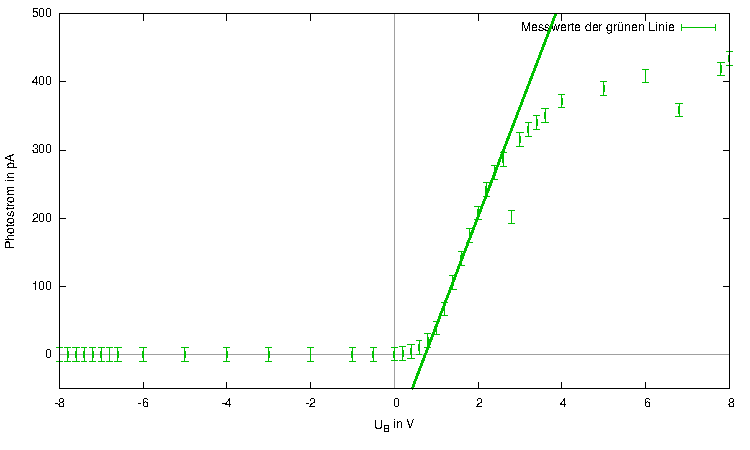
\includegraphics[width=\textwidth]{graphen/3b}}
\captionof{figure}{Kennlinie der grünen Linie}
\end{minipage}
\begin{minipage}{\linewidth}
\centering
\makebox[0cm]{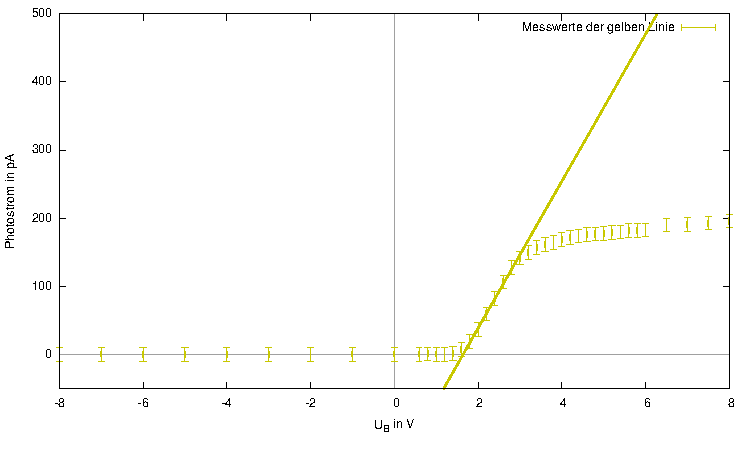
\includegraphics[width=\textwidth]{graphen/3c}}
\captionof{figure}{Kennlinie der gelben Linie}
\end{minipage}
\end{center}
Durch lineare Regression von den als linear empfunden Werten wurden folgende Parameter für Steigung \(b\) und Ordinaten-abschnitt \(a\) ermittelt:
\begin{center}
\begin{tabular}{c|ccc}
		& \(b\) & \(a\) & linearer Bereich (\(U_B\))\\\hline
Indigo  & \((37,0 \pm 1,0)\frac{pA}{V}\) & \((1,8 \pm 1,7)\,pA\) & \((0,5 - 2,5)\,V\)\\
grün    & \((37,0 \pm 1,0)\frac{pA}{V}\) & \((1,8 \pm 1,7)\,pA\) & \((1 - 2,5)\,V\)\\
gelb    & \((37,0 \pm 1,0)\frac{pA}{V}\) & \((1,8 \pm 1,7)\,pA\) & \((2 - 3)\,V\)
\end{tabular}
\end{center}
\subsubsection{Auswertung}
Aus den ermittelten Parametern können nun die Grenzspannungen errechnet werden:
\begin{align}
I_{Pho}(U) &= a + b \cdot U \\
I_{Pho}(U_{grenz}) &= 0 = a + b \cdot U_{grenz}\\
\Rightarrow U_{grenz} &= - \frac{a}{b}\\
\Rightarrow \Delta U_{grenz} &= U_{grenz} \cdot \sqrt{
\left( \frac{\Delta a}{a} \right)^2 +
\left( \frac{\Delta b}{b} \right)^2
}
\end{align}
Außerdem gilt für das Verhältnis von Wellenlängen und Frequenzen:
\begin{equation}
f = \frac{c}{\lambda}
\end{equation}
Wobei c die Lichtgeschwindigkeit \(2,99 \cdot 10^8\,\frac{m}{s}\) bezeichnet.

Somit ergben sich 3 Wertepaare \((f, U_{grenz})\) für jeden Graphen:
\begin{center}
\begin{tabular}{c|c}
\(f\, [10^{14}\, Hz]\) & \(U_{grenz}\, [V]\) \\\hline
\(6,88\) & \(0,05 \pm 0,94\) \\
\(5,49\) & \(-0,738 \pm 0,075\) \\
\(5,20\) & \(-1,642 \pm 0,068\) \\
\end{tabular}
\captionof{table}{Wertepaare (f,U)}
\end{center}
Nunwerden diese Wertepaare graphisch aufgetragen:
\begin{center}
\begin{minipage}{\linewidth}
\centering
\makebox[0cm]{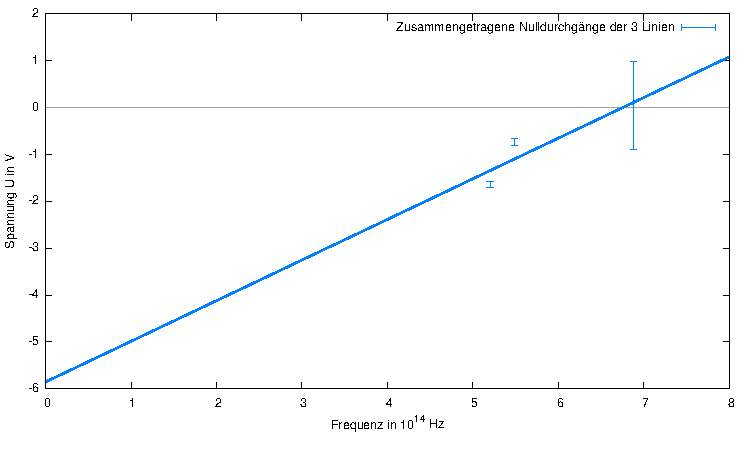
\includegraphics[width=\textwidth]{graphen/h}}
\captionof{figure}{U gegen f aufgetragen}
\end{minipage}
\end{center}
Durch das graphische aufgetragen erhält man für die Parameter:
\begin{align}
b &= (0,87 \pm 0,37)\, \frac{V s}{10^{14}}\\
a &= (-5,9 \pm 2,2)\, V
\end{align}
Für die Energie eines Lichtquants gilt:
\begin{equation}
E = h \cdot f
\end{equation}
Und da eine Austrittsarbeit \(W_A\) geleistet werden muss um ein Elektron aus einem Leiter zu lösen gilt:
\begin{equation}
T = E - W_A
\end{equation}
Die Kinetische Energie \(T\) wird, wenn die Grenzspannung angelegt ist im Elektrischen Feld Umgesetzt, daher gilt
\begin{align}
T &= e \cdot U_{grenz}\\
\Rightarrow e \cdot U_{grenz} &= h \cdot f - W_A \\
U_{grenz} &= \frac{h}{e} \cdot f - \frac{W_A}{e} 
\end{align}
,wobei \(e\) die Ladung des Elektrons \(1,60 \cdot 10^{-19} \, C\) bezeichnet.
Es kann nun \(W_A\) als \(-a\cdot e\) und \(h\) als \(b\cdot e\) identifiziert werden.
Es ergibt sich:
\begin{align}
h &= (13,9 \pm 5,9)\, 10^{-34} Js \\
W_A &= (9,4 \pm 3,5)\, 10^{-19} J
\end{align}
\subsubsection{Fazit}
Der Versuch war leicht durchführbar und die Messung lieferte stetige Werte. Die Messung ist dennoch nicht sehr zuverlässig gewesen, da schon durch leichte Erschütterungen der Optische Aufbau wackelte und der Strahlengang nicht mehr zentral auf den Detektor traf. Außerdem konnte nicht garantiert werden, dass die Einzelnen Linien mittig auf den Detektor ausgerichtet wurden. Die Selbstgebaute Apparatur sichert außerdem nicht, das Die Elektroden nur aus einem Reinen Metall gefertigt sind, auffällig ist nämlich, dass auch ein Anoden-Kathoden-Strom bei Gegenspannungen messbar war, was jedoch auch an der Kalibrierung des Messgeräts liegen könnte. Die Wertepaare für \(U_{grenz}\) und \(f\) bilden keinen wirklich erkennbar linearen verlauf. Das Modell kann dahingehend also nicht bestätigt werden, und es ist von einem großen systematischen Fehler auszugehen Für die Austrittsarbeit steht aufgrund der Unbekanntheit des Kathodenmaterials kein Vergleichswert zur Verfügung. Der Wert für das Plancksche Wirkungsquantum \(h\) ist verträglich mit dem Literaturwert, da die dreifachen Fehlerintervalle überlappen:
\begin{center}
\begin{tabular}{c|c}
Messung & Literatur \\\hline
\((13,9 \pm 5,9)\cdot 10^{-34} \,Js \) & \( 6,626 \cdot 10^{-34}\, Js\)
\end{tabular}
\captionof{table}{Endresultat für h}
\end{center}